\chapter{Ordinary Differential Equations}

In the previous chapter, we found the equilibrium point where a duck would float on water.  This kind of problem is called {\em static} because it does not move.  In this chapter I introduce {\em dynamic} problems, which involve things that change over time.
 
Also, you'll learn about a mathematical tool for describing physical systems, {\em differential equations}, and two computation tools for solving them, Euler's method and {\tt ode45}.

But first I have a quick suggestion about organizing code in files.

\section{Functions and Files}
\label{funfiles}

So far we've only put one function in each file.  It's also possible
to put more than one function in a file, but only the first one, the
{\em top-level function}, can be called from the Command
Window.  The other {\em helper functions} can be called from anywhere inside the file, but not from the Command Window or any other file.

\index{function!top-level}
\index{top-level function}
\index{helper function}
\index{function!helper}

Keeping multiple functions in one file is convenient, but it makes debugging
difficult because you can't call helper functions from the Command
Window.

To help with this problem, I often use the top-level function
to develop and test my helper functions.  For example, to write
a program for Exercise~\ref{duck}, I would create a file named
{\em duck.m} and start with a top-level function named {\tt duck}
that takes no input variables and returns no output value.

Then I would write a function named \verb"error_func" to
evaluate the error function for {\tt fzero}.  To test
\verb"error_func" I would call it from {\tt duck} and then
call {\tt duck} from the Command Window.

\index{incremental development}

Here's what my first draft might look like:

\begin{code}
function res = duck()
    error = error_func(10)
end

function res = error_func(d)
    rho = 0.3;      % density in g / cm^3
    r = 10;         % radius in cm
    res = d;
end
\end{code}

The line {\tt res = d} isn't finished yet, but this
is enough code to test.
Once I finished and tested \verb"error_func", I would modify
{\tt duck} to use {\tt fzero}.

This problem might only require two functions, but if there
were more, I could write and test them one at a time, and then
combine them into a working program.

Now, let's get back to differential equations.


\section{Differential Equations}
\label{diffeq}

A {\em differential equation} (DE) is an equation that describes the
derivatives of an unknown function.  ``Solving a DE'' means finding a
function whose derivatives satisfy the equation.

\index{differential equation}
\index{equation!differential}

For example, suppose we would like to predict the population of yeast growing in a nutrient solution.  Assume that we know the initial population is 5 billion yeast cells.

When yeast grow in particularly yeast-friendly
conditions, the rate of growth at any point in time is proportional to the current population.  If we define $y(t)$ to be the population at  time $t$, we can write the following equation for the rate of growth:
%
\begin{equation}
\frac{dy}{dt}(t) = a y(t)
\end{equation}
%
where $\frac{dy}{dt}(t)$ is the derivative of $y(t)$ and
$a$ is a constant that characterizes how quickly the population
grows.
This equation is ``differential'' because it relates a function to one of its derivatives.

\index{ordinary differential equation}

It is an {\em ordinary} differential equation (ODE) because all the
derivatives involved are taken with respect to the
same variable.
If it related derivatives with respect to
different variables (partial derivatives), it would be a {\em partial}
differential equation.

\index{first-order differential equation}

This equation is {\em first-order} because it involves only first
derivatives.  If it involved second derivatives, it would be second order,
and so on.

\index{linear differential equation}

Lastly, it's \emph{linear} because each term involves $t$, $f$, or
$df/dt$ raised to the first power; if any of the terms involved
products or powers of $t$, $f$, and $df/dt$ it would be
nonlinear.

Now suppose we want to predict the yeast population in the future.  We can do that using Euler's method.

\section{Euler's Method}

Here's a test to see if you're as smart as Euler.  Let's say you arrive at time $t$ and measure the current population, $y$, and
the rate of change, $r$.  What do you think the population will
be after some period of time $\Delta t$ has elapsed?

If you said $y + r \Delta t$, congratulations!  You just invented
Euler's method.

\index{Euler's Method}

This estimate is based on the assumption that $r$ is constant, but
in general it's not, so we only expect the estimate to be good if
$r$ changes slowly and $\Delta t$ is small. 

What if we want to make a prediction when $\Delta t$ is large?
One option is to break $\Delta t$ into smaller pieces, called
{\em time steps}. Then we can use the following equations to get from one time step to the next:

\begin{eqnarray}
T_{i+1} &=& T_i + dt                       \\
Y_{i+1} &=& Y_i + \frac{df}{dt}(t)~dt          
\end{eqnarray}

Here $\{T_i\}$ is a sequence of times where we estimate the value
of $y$, and $\{Y_i\}$ is the sequence of estimates.  For each
index $i$, $Y_i$ is an estimate of $y(T_i)$.

\index{time step}

If the rate doesn't change too fast and the time step isn't
too big, Euler's method is accurate enough for most purposes.  

%One
%way to check is to run it once with time step $dt$ and then run it
%again with time step $dt/2$.  If the results are the same, they are
%probably accurate, as . . .; otherwise, we can cut the time step again.


\section{Implementing Euler's method}

As an example I'll use Euler's method to solve the equation from ``\nameref{diffeq}'':

\[ \frac{dy}{dt}(t) = a y(t) \]

with the initial condition $y(0) = 5$ billion cells and
the growth parameter $a = 0.2$ per hour. 

\index{top-level function}

As a first step, I created a file named {\em euler.m} with a top-level function and a helper function:

\begin{code}
function res = euler()
    T(1) = 0;
    Y(1) = 5;
    r = rate_func(T(1), Y(1))
end

function res = rate_func(t, y)
   a = 0.2;
   dydt = a * y;
   res = dydt;
end
\end{code}

In {\tt euler} I initialize the initial conditions and then call \verb"rate_func", so called because it computes the rate of growth in the population.

\index{initial condition}

After testing these functions, I added code to {\tt euler} to compute these difference equations:

\begin{eqnarray}
T_{i+1} &=& T_i + \Delta t             \\
Y_{i+1} &=& Y_i + r \Delta t          
\end{eqnarray}
%
where $r$ is the rate of growth computed by \verb"rate_func".
Listing~\ref{lst:euler_method} has the code we need:

\begin{lstlisting}[caption={A function implementing Euler's method}, label={lst:euler_method}]
function res = euler()
    T(1) = 0;
    Y(1) = 5;
    dt = 0.1;
    
    for i=1:40
        r = rate_func(T(i), Y(i));
        T(i+1) = T(i) + dt;
        Y(i+1) = Y(i) + r * dt;
    end
    plot(T, Y)
end
\end{lstlisting}

Before the loop, we create two vectors, {\tt T} and {\tt Y}, and set the first element of each with the initial conditions.  {\tt dt}, which is the size of the time steps, is 0.1 hours.

Inside the loop, we compute the growth rate based on the current time, {\tt T(i)}, and population, {\tt Y(i)}.  You might notice that the rate depends only on population, but I pass time as an input variable anyway, for reasons you'll see soon.

After computing the growth rate, we add an element to each of {\tt T} and {\tt Y}.  Then, when the loop exits, we plot {\tt Y} as a function of {\tt T}.

If you run the code, you should get a plot of population over time, shown in Figure~\ref{fig:euler}. 

\begin{figure}[ht]
\centerline{\includegraphics[height=3in]{book/figs/euler.eps}}
\caption{Solution to a simple differential equation by Euler's method.}
\label{fig:euler}
\end{figure}

As you can see, the population doubles in a little less than 4 hours.


\section{Solving ODEs with ode45}
\label{ode45}

A limitation of Euler's method is that it assumes that the derivative is constant between time steps, and that's not generally true.  Fortunately, there are better methods that estimate the derivative between time steps, and they are much more accurate.

\index{time step} 
\index{ode45@{\tt ode45}}

MATLAB provides a function called {\tt ode45} that implements one of these methods.  In this section I'll explain how to use it; you can read more about how it works in ``\nameref{howode45}'' on page~\pageref{howode45}.

\index{rate function}
\index{function!rate}

In order to use {\tt ode45}, you have to write a function that evaluates $dy/dt$ as a function of $t$ and $y$.  Fortunately, we already have one, called \verb"rate_func":

\begin{code}
function res = rate_func(t, y)
   a = 0.2;
   dydt = a * y;
   res = dydt;
end
\end{code}

We can call {\tt ode45} from the Command Window like this:

\begin{code}
[T, Y] = ode45(@rate_func, [0, 4], 5);
plot(T, Y)
\end{code}

The first argument is a function handle, as we saw in Chapter~\ref{fzero}.  The second argument is the time interval where we want to evaluate the solution; in this case the interval is from $t=0$ to $t=4$ hours.  The third argument is the initial population, 5 billion cells.

\index{function handle}
\index{handle!function}
\index{output variable}
\index{variable!output}

{\tt ode45} is the first function we've seen that returns {\em two} output variables.
In order to store them, we have to assign them to two variables, {\tt T} and {\tt Y}.

\begin{figure}[ht]
\centerline{\includegraphics[height=3in]{book/figs/runge.eps}}
\caption{Solutions to a simple differential equation using Euler's method and {\tt ode45}.}
\label{fig:runge}
\end{figure}

Figure~\ref{fig:runge} shows the results.  The solid line is the estimate we computed with Euler's method; the dashed line is the solution from {\tt ode45}.

For the first 2-3 hours, the two solutions are visually indistinguishable.  During the last hour, they diverge slightly; at 4 hours, the difference is less than 1\%.

For many purposes, the difference between Euler's method and {\tt ode45} is the least of our worries.  In this example, we probably don't know the initial population with perfect accuracy, or the growth constant, {\tt a}.  Also the assumption that the growth rate only depends on population is probably not true.  Any of these modeling errors could be bigger than 1\%.

However, for some problems, Euler's method can be off by a lot more than 1\%.  
In those cases {\tt ode45} is almost always more accurate, for two reasons: first, it computes the rate function several times per time step; also, if the time step is too big, {\tt ode45} can detect the problem and shrink the time step.  For more details, see ``\nameref{howode45}'' on page~\pageref{howode45}.


\section{Time Dependence}

Looking at \verb"rate_func" in the previous section, you might notice that it takes {\tt t} as an input variable, but doesn't use it.  That's because the growth rate does not depend on time---bacteria don't know what time it is.

\index{time dependence}

But rats do.  Or, at least, they know what season it is.
Suppose that the growth rate for rats depends on the current population {\em and} the availability of food, which varies over the course of the year.
The differential equation might be something like
%
\begin{equation}
\frac{dy}{dt}(t) = a y(t) \left(1 - \cos (\omega t) \right)
\end{equation}
%
where $t$ is time in days and $y(t)$ is the population at time $t$.

$a$ and $\omega$ are {\em parameters}, which are values that
quantify a physical aspect of the scenario.  Parameters are often constants, but in some models they vary in time.

\index{parameter}

In this example, $a$ characterizes the reproductive rate per day, and
$\omega$ is the frequency of a periodic function that describes
the effect of varying food supply on reproduction.

We'll use the values $a = 0.002$
and $\omega = 2 \pi/365$ (one cycle per year).
The growth rate is lowest at $t=0$, on January 1, and highest at $t=365/2$, on June 1.

Now we can write a function that evaluates the growth rate:

\begin{code}
function res = rate_func(t, y)
    a = 0.002;
    omega = 2*pi / 365;
    res = a * y * (1 - cos(omega * t));
end
\end{code}

To test this function, I put it in a file called {\em rats.m} with a top-level function called 
{\tt rats}:

\begin{code}
function res = rats()
    t = 365/2;
    y = 1000;
    res = rate_func(t, y);
end
\end{code}

The top-level function assumes as an example that
there are 1000 rats at $t=365/2$ (June 31).  Then it computes the growth rate under those considitions.

We can run the top-level function like this:

\begin{code}
>> ***r = rats***

r = 4
\end{code}

Under these conditions, the growth rate is 4 new rats per day. 

Now that we've tested \verb"rate_func", we can use {\tt ode} to solve the differential equation.
Here's how to call it from the top-level function in {\em rats.m}):

\begin{code}
[T, Y] = ode45(@rate_func, [0, 365], 1000)
plot(T, Y)
\end{code}

The first argument is a function handle, again.  The second argument is the interval we are interested in, a duration of one year, expressed in units of days.
The third argument is the initial population, $y(0) = 1000$.

\index{interval}

Figure~\ref{fig:rats} shows the results. 

\begin{figure}[ht]
\centerline{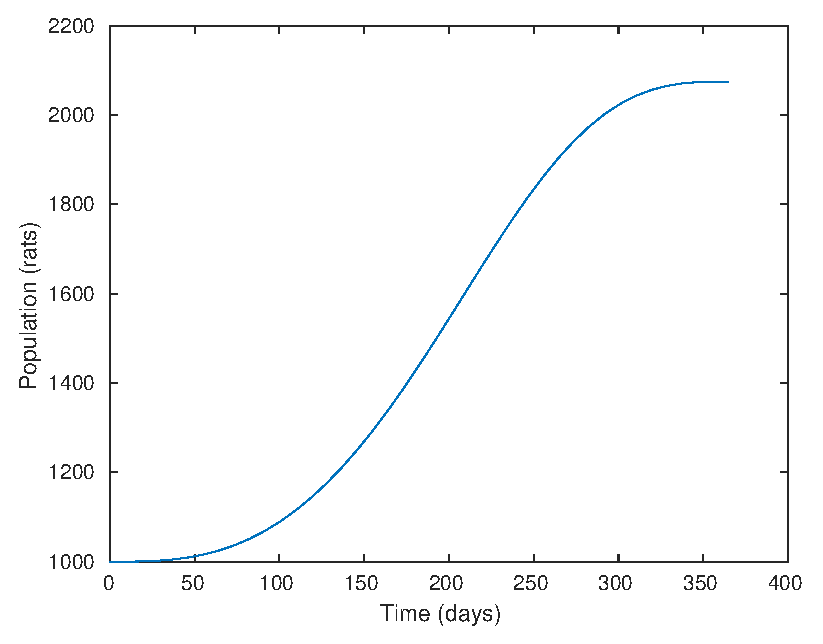
\includegraphics[height=3in]{book/figs/rats.eps}}
\caption{Solutions to a simple differential equation by Euler's method and {\tt ode45}.}
\label{fig:rats}
\end{figure}

The population grows slowly during the winter, quickly during the summer, and the slowly again in the fall.

To see the population at the end of the year, you can display the last element of {\tt Y}:

\begin{code}
Y(end)
2.0751e+03
\end{code}

That's a little more than 2000 rats, so the population roughly doubles in one year.

The index is {\tt end}, which is a special word in MATLAB that means ``the index of the last element''.  You can use it in an expression, so {\tt Y(end-1)} is the second-to-last element of
{\tt Y}.

\index{end@{\tt end}}
\index{index!{\tt end}}


\section{What Could Go Wrong?}

Don't forget the {\tt @} on the function handle.
If you leave it out, like this:

\begin{code}
[T, Y] = ode45(rate_func, [0, 365], 1000)
\end{code}

MATLAB treats the first argument as a function
call and calls \verb"rate_func" without providing arguments.
Then you get an error message:

\index{rate function}
\index{function handle}

\begin{code}
Not enough input arguments.

Error in rats>rate_func (line 18)
    res = a * y * (1 - cos(omega * t));

Error in rats (line 6)
    [T, Y] = ode45(rate_func, [0, 365], 1000);
\end{code}

Also, the rate function you write has to take two input variables, 
{\tt t} and {\tt y}, in that order, and return one output variable, 
{\tt res}.

\index{output variable}

If you're working with a rate function like this:

\begin{equation}
\frac{dy}{dt}(t) = a y(t)
\end{equation}

You might be tempted to write this:

\begin{code}
function res = rate_func(y)        % WRONG
    a = 0.002;
    res = a * y;
end
\end{code}

But that would be wrong.  So very wrong.  Why?  Because
when {\tt ode45} calls \verb"rate_func", it provides two arguments.
If you only take one input variable, you'll get an error.  So
you have to write a function that takes {\tt t} as an input
variable, even if you don't use it.

\index{input variable}

\begin{code}
function res = rate_func(t, y)     % RIGHT
    a = 0.002;
    res = a * y;
end
\end{code}

Another common error is to write a function that doesn't make
an assignment to the output variable.  If you write something
like this:

\begin{code}
function res = rate_func(t, y)
    a = 0.002;
    omega = 2*pi / 365;
    r = a * y * (1 - cos(omega * t));    % WRONG
end
\end{code}

And then call it from {\tt ode45}, you get

\begin{code}
Output argument "res" (and maybe others) not assigned during call
to "rate_func".
\end{code}

I hope these warnings save you some time debugging.

\section{Labeling Axes}

The plots in this chapter have labels on the axes, and one of them has a legend, but I didn't show you how to do that.  Let's do it now.

\index{labeling axes}
\index{axes}
\index{xlabel@{\tt xlabel}}
\index{ylabel@{\tt ylabel}}

The functions to label the axes are {\tt xlabel} and {\tt ylabel}:

\begin{code}
xlabel('Time (hours)')
ylabel('Population (billions of cells)')
\end{code}

The function to generate a legend is {\tt legend}:

\begin{code}
legend('euler', 'ode45')
\end{code}

\index{legend@{\tt legend}}

The arguments are the labels for the lines, in the order they were drawn.  Usually the legend is in the upper right corner, but you can move it by providing an optional argument called {\tt Location}:

\begin{code}
legend('euler', 'ode45', 'Location', 'northwest')
\end{code}

Finally, I saved the figures using {\tt saveas}:

\begin{code}
saveas(gcf, 'runge.eps', 'epsc')
\end{code}

The first argument is the figure we want to save; {\tt gcf} is a MATLAB command that stands for ``get current figure'', which is the figure we just drew.  The second argument is the filename.  The extension specifies the format we want, which is Encapulated PostScript.  The third argument tells MATLAB what ``driver'' to use.  The details aren't important, but {\tt epsc} generates figures in color.

\index{figure}
\index{get current figure}
\index{gcf@{\tt gcf}}
\index{saveas@{\tt saveas}}

\section{Chapter Review}

In this chapter I defined a differential equation (DE) as an equation that relates the
derivatives of an unknown function.  
In an ordinary DE (ODE), all derivatives are taken with
respect to the same variable, as opposed to a partial DE (PDE), which includes derivatives with respect to more than one variable

A {\em first-order DE} includes only first derivatives, and a {\em linear DE} includes no products or powers of the function and its derivatives.
A differential equation is {\em time dependent} if the rate function depends on time.

When we solve a differential equation numerically, the {\em time step} is the interval in time between successive elements of the solution.
A {\em parameter} is a value that appears in a model to quantify some
physical aspect of the scenario being modeled.

Until now we have only put one function in each M-file, but in this chapter we wrote a {\em top-level function}, which is the first function in an M-file and a {\em helper function} which is any function in an M-file that is not the top-level function.

In the next chapter we'll solve {\em systems} of ODEs, which are used to describe physical systems with multiple parts that interact.
But first, here's an exercise where you can apply what you've learned so far.


\section{Exercises}

\begin{ex}

\index{coffee}
\index{cooling}
\index{Newton's law of cooling}

Suppose that you're given an 8 ounce cup of coffee at \SI{90}{\celsius}.
You have learned from bitter experience that the hottest coffee you
can drink comfortably is \SI{60}{\celsius}.  

If the temperature of the coffee drops by \SI{0.7}{\celsius} during the first minute, how long will you have to wait to drink your coffee?

You can answer this question with Newton's Law of Cooling (See \url{https://greenteapress.com/matlab/newton}).:
%
\begin{equation*}
\frac{dy}{dt}(t) = -k (y(t) - e)
\end{equation*}
%
where $y(t)$ is the temperature of the coffee at time $t$,
$e$ is the temperature of the environment, and $k$ is a parameter
that characterizes the rate of heat transfer from the coffee from the environment.

Let's assume that $e$ is \SI{20}{\celsius} and constant; that is, the coffee does not warm up the room.

Let's also assume $k$ is constant.  In that case, we can estimate it based on the information we have.  If the temperature drops \SI{0.5}{\celsius} during the first minute, when the coffee is \SI{90}{\celsius}, we can write
%
\begin{equation*}
-0.7 = -k (90 - 20)
\end{equation*}
%
Solving this equation yields $k = 0.01$.

Here are some suggestions for getting started:

\begin{itemize}

\item Create a file named {\em coffee.m} and write a function
called {\tt coffee} that takes no input variables.  Put a simple statement like {\tt x=5} in the body of the function and invoke {\tt coffee} from the Command Window.

\item Add a helper function called \verb"rate_func" that takes {\tt t} and {\tt y} and computes $\frac{dy}{dt}$.  In this case \verb"rate_func" does not actually depend on $t$; nevertheless, your function has to take $t$ as the first input variable in order to work with {\tt ode45}.

\item Test your function by adding a line like \verb"rate_func(0, 90)"
to {\tt coffee}, then call {\tt coffee} from the {\sf Command Window}.
Confirm that the initial rate is \SI{-0.7}{\celsius \per \minute}.

\item Once you get \verb"rate_func" working, modify
{\tt coffee} to use {\tt ode45} to compute the temperature
of the coffee for 60 minutes.  Confirm that
the coffee cools quickly at first, then more slowly, and reaches
room temperature after about an hour.

\item Plot the results and estimate the time when the temperature reaches \SI{60}{\celsius}.

\end{itemize}

\end{ex}




